\documentclass[a4paper]{report}
\usepackage[group-separator={,},group-minimum-digits={3}]{siunitx}
\usepackage[utf8]{inputenc}
\usepackage[dvipsnames]{xcolor}
\usepackage{tcolorbox}
\usepackage{multicol}
\usepackage{lipsum}
\usepackage[margin=0.2in]{geometry}
\usepackage{xstring}
\usepackage{xifthen}
\usepackage[dvipsnames]{xcolor}
\usepackage{setspace}
\usepackage{amsmath}
\usepackage{enumitem}
\pagenumbering{gobble}
\setlength{\columnsep}{1.5cm}
\setlength{\columnseprule}{0.2pt}
\usepackage{hyperref}
\usepackage[none]{hyphenat}
\usepackage{graphicx}
\usepackage{etoolbox}
\usepackage{titlepic}
\usepackage{enumitem}

\setlist{nosep}

\hypersetup{
    colorlinks,
    citecolor=black,
    filecolor=black,
    linkcolor=black,
    urlcolor=black
}

\makeatletter
\def\@makechapterhead#1{%
  %\vspace*{5\p@}%
  {\parindent \z@ \raggedleft \normalfont
    \ifnum \c@secnumdepth >\m@ne
        \large\bfseries #1
        \par\nobreak
%        \vskip 10\p@
        \rule{\columnwidth}{.1pt}%
%        \vskip 10\p@
    \fi
    \interlinepenalty\@M
%    \large \bfseries \MakeUppercase{#1}\par\nobreak
%    \vskip 5\p@
  }}
\makeatother

\usepackage{enumitem}
\setitemize{noitemsep,topsep=0pt,parsep=0pt,partopsep=0pt}
\usepackage{graphicx}
\title{Fire Emblem Awakening Any\% Normal/Classic}
\author{Mr.Tyton}
\titlepic{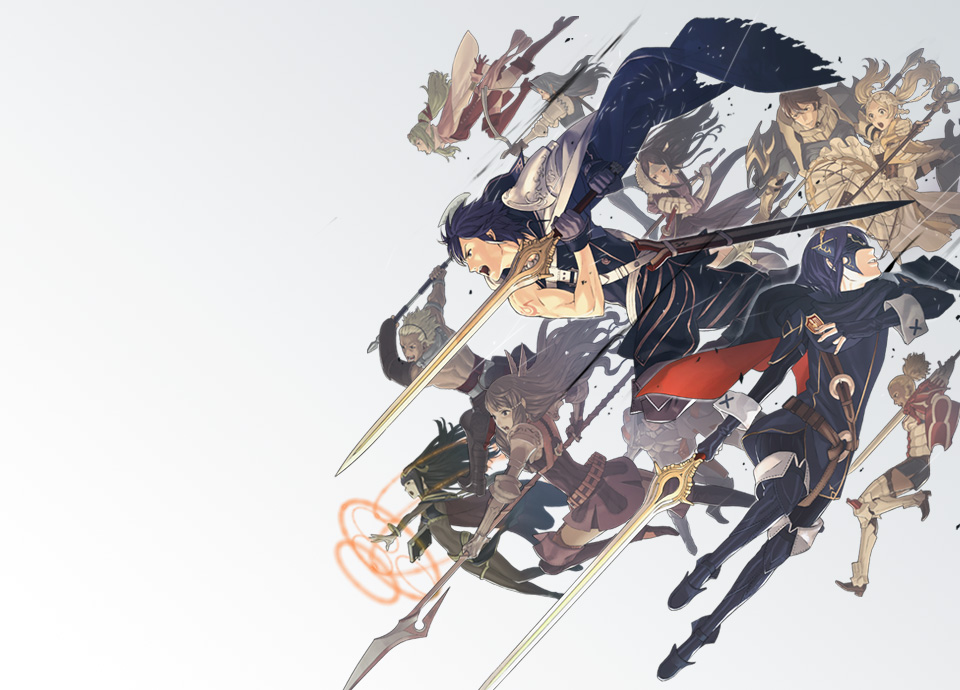
\includegraphics[width=\textwidth]{fire_emblem_awakening_logo.jpg}}
\begin{document}
\singlespacing
\maketitle
\makeatletter
\patchcmd{\chapter}{\if@openright\cleardoublepage\else\clearpage\fi}{}{}{}
\makeatother

\newcounter{chaptercount}

\newenvironment{battlespecial}[1]{\begin{tcolorbox}[title=\begin{center}#1\end{center},colbacktitle=red!50!white]}{\end{tcolorbox}}
\newenvironment{battle}[1]{\refstepcounter{chaptercount} \begin{tcolorbox}[title=\begin{center}Chapter \thechaptercount\ - #1\end{center},colbacktitle=red!50!white]}{\end{tcolorbox}}


\newcommand{\battleinfo}[3]{Goal: \ifthenelse{\equal{#1}{rout}}{Rout the Enemy}{\ifthenelse{\equal{#1}{commander}}{Defeat the Commander}{#1}} \newline Turns: #2 \newline Units: #3}


\newenvironment{shop}[1]{\begin{tcolorbox}[title=\begin{center}SHOP\, #1 GOLD\end{center},colbacktitle=OliveGreen!50!white]}{\end{tcolorbox}}

\newcommand{\cs}[1][]{\textbf{CS}%
	\ifthenelse{\isempty{#1}}{}{ (#1)}%
}

\setlist[enumerate]{label={Turn \arabic*:\newline}, align=left}
%\setlist[itemize]{align=left}

\newcommand{\robin}{\textbf{\textcolor{purple}{Robin}}}
\newcommand{\anna}{\textbf{\textcolor{green}{Anna}}}
\newcommand{\chrom}{\textbf{\textcolor{blue}{Chrom}}}
\newcommand{\lucina}{\textbf{\textcolor{cyan}{Lucina}}}
\newcommand{\frederick}{\textbf{\textcolor{gray}{Frederick}}}
\newcommand{\sully}{\textbf{\textcolor{BrickRed}{Sully}}}
\newcommand{\cordelia}{\textbf{\textcolor{Mahogany}{Cordelia}}}
\newcommand{\ricken}{\textbf{\textcolor{Emerald}{Ricken}}}
\newcommand{\nowi}{\textbf{\textcolor{SpringGreen}{Nowi}}}
\newcommand{\olivia}{\textbf{\textcolor{Magenta}{Olivia}}}
\newcommand{\cherche}{\textbf{\textcolor{Maroon}{Cherche}}}
\newcommand{\sayri}{\textbf{\textcolor{PineGreen}{Say'ri}}}
\newcommand{\basilio}{\textbf{\textcolor{brown}{Basilio}}}
\newcommand{\flavia}{\textbf{\textcolor{RawSienna}{Flavia}}}
\newcommand{\enemy}[1]{\textbf{\textcolor{red}{#1}}}


\newcommand{\autoturn}{\turn{\auto}}
\newcommand{\autoblitz}{\item Set Auto to \textbf{Blitz}}
\newcommand{\autocustom}{\item Set Auto to \textbf{Custom}}
\newcommand{\auto}{\item Auto}
\newcommand{\pair}[2]{\item Pair #1 to #2}
\newcommand{\move}[1]{\item Move #1}
\newcommand{\attack}[2]{\item Attack \enemy{#1} #2}
\newcommand{\attacks}[2]{\ Attack \enemy{#1} #2}
\newcommand{\wait}{\item Wait}
\newcommand{\turn}[1]{\item \ \begin{itemize} #1 \end{itemize}}
\newcommand{\turnend}{\item End}
\newcommand{\trade}[3]{\item Trade with #1: #2 for #3}
\newcommand{\use}[1]{\item Use #1}
\newcommand{\equip}[1]{\item Equip #1}
\newcommand{\movewait}[1]{\begin{itemize}\move{#1}\wait\end{itemize}}
%\newcommand{\movewait}[1]{\ Move [{#1}], Wait}
\newcommand{\moveuse}[2]{\begin{itemize}\move{#1}\use{#2}\end{itemize}}
\newcommand{\moveequip}[2]{\begin{itemize}\move{#1}\equip{#2}\wait\end{itemize}}
\newcommand{\moveattack}[3]{\begin{itemize}\move{#1}\attack{#2}{#3}\end{itemize}}
\newcommand{\map}[1]{\item View Map: \begin{itemize}#1\end{itemize}}
\newcommand{\swap}[2]{\item Switch #1 with #2}

\newcommand{\dance}[3]{\oliviaf \begin{itemize}\move{#1}\item Dance for #2 #3\end{itemize}}
\newcommand{\rally}[1]{\lucinaf \begin{itemize}\move{#1}\item Rally\end{itemize}}

\newcommand{\units}[1]{\item Select Units: \begin{itemize} #1 \end{itemize}}
\newcommand{\remove}[1]{\item Remove #1}
\newcommand{\add}[1]{\item Add #1}
\newcommand{\safetysave}{\item This is a good time to Safety \textbf{Save}}

\newcommand{\prep}[1]{\newline\newline Preparations: \begin{itemize} #1 \end{itemize}}
\newcommand{\inventory}[1]{\item Inventory: \begin{itemize} #1 \end{itemize}}

\newcommand{\support}[3]{\item Support #1 to #2, Rank #3}

\newcommand{\robinf}{\item \robin:}
\newcommand{\chromf}{\item \chrom:}
\newcommand{\frederickf}{\item \frederick:}
\newcommand{\lucinaf}{\item \lucina:}
\newcommand{\sullyf}{\item \sully:}
\newcommand{\rickenf}{\item \ricken:}
\newcommand{\cordeliaf}{\item \cordelia:}
\newcommand{\nowif}{\item \nowi:}
\newcommand{\oliviaf}{\item \olivia:}
\newcommand{\cherchef}{\item \cherche:}
\newcommand{\sayrif}{\item \sayri:}
\newcommand{\basiliof}{\item \basilio:}
\newcommand{\flaviaf}{\item \flavia:}


\setlength{\columnsep}{.5cm}

\section*{Acknowledgements}

Thank you to the people on the FE Discord, including but not limited to: \textbf{Yukiya}, \textbf{Quo}, \textbf{ShockraTease}.

\section*{Introduction}

Original notes can be found in this link: \url{https://goo.gl/kw4XWT}
\newline\newline
\textbf{\large{General Notes and Tips}}
\newline\newline
\begin{itemize}
    \item There’s no RNG manipulation in this run. As such, you can feel free to do whatever cursor movement you like.
    \item All X/Y switching strategies in this route are up to personal preference, though generally speaking you want to at least follow the order of characters used each turn.
    \item These notes assume fixed growths mode where the stats of characters are always the same, assuming you follow the route. The route will not be consistent nor hold if you decide to run random mode. More details about fixed growths can be found \href{https://serenesforest.net/path-of-radiance/general/fixed-mode/}{here}.
    \item Don’t skip cutscenes for opening chests, this is slower than letting them play out.
    \item Do skip cutscenes for opening doors, though.
    \item Cursor Movement - You should be holding B anytime you select and move the cursor for longer distances. Hold B before selecting a character so you don’t accidentally cancel.
    \begin{itemize}
        \item D-pad is useful for straight rigid movement. The cursor will always be stopped by terrain / enemy units and the current character’s movement range.
        \item Analog stick is useful for diagonal movement and/or moving through terrain, since the analog stick will never be stopped by terrain / enemy units. However, it also isn’t stopped by the character’s movement range.
    \end{itemize}
    \item You should be doing the FEP (Fast Enemy Phase) glitch on every turn in the run (this makes the camera move more quickly between non-player units, saving minutes overall).
    \begin{itemize}
        \item Holding B as your last action ends, then opening the menu and ending turn while holding B should always work.
        \item If you did a character movement without holding B, it’s better to open the main menu while holding B and a direction (like FEP in radiant dawn).
    \end{itemize}
    \item On Enemy Phase, holding down the A button will make it so the white box around a character will not appear.
    \item Mashing A and Start clears the exp bar faster (both in a level and bonus exp in base).
    \item Mashing start clears the level up screen faster.
    \item X = do an X-switch.
    \begin{itemize}
        \item Pressing X on a character will jump the cursor to the next unused character in the unit list.
        \item Pressing X on an empty tile will jump the cursor to the top unused character in the unit list.
        \item You should be holding B during all X switches so the camera move quickly.
        \item Note abbreviations for X-switching:
        \begin{itemize}
            \item “2X” = press X twice to jump to Character
            \item “Off X” = press X on an empty tile to jump to Character
            \item “X on Character1” = move cursor to Character1, press X to jump to Character2
        \end{itemize}
    \end{itemize}
    \item Y = do a Y-switch.
    \begin{itemize}
        \item Pressing Y on a character brings up the character screen. This is primarily useful for going backwards in the unit list since it skips moving the camera when you cancel. For example, if the top of the Unit List is Ike, Marcia, Tanith, and you want to select Marcia after moving Tanith, you press Y on Tanith, press up once, then press B to instantly select Marcia.
    \end{itemize}
\end{itemize}
\newpage

\begin{multicols}{2}
Avatar Setup:
\begin{itemize}
	\item Female
	\item Asset: Magic
	\item Flaw: Defense
\end{itemize}
\begin{battlespecial}{Premonition - Invisible Ties}
\battleinfo{rout}{2-3}{\chrom, \robin}
\begin{enumerate}
\item \ 
\begin{itemize}
\item Options:
\begin{itemize}
\item Combat Animations: \textbf{OFF}
\item Other Animations: \textbf{OFF}
\item Game Speed: \textbf{FAST}
\item Skip Actions: \textbf{ALL}
\item Confirm Auto: \textbf{NO}
\end{itemize}
\autoblitz
\auto
\end{itemize}
\autoturn
\end{enumerate}
\end{battlespecial}
\begin{battlespecial}{Prologue - The Verge of History}
\battleinfo{rout}{4}{\chrom, \robin}
\begin{enumerate}
\item \ 
\begin{itemize}
\pair{\chrom}{\robin}
\auto
\end{itemize}
\item \ 
\begin{itemize}
\item Set Auto to Custom; \robin\ to \textbf{Blitz}
\auto
\end{itemize}
\autoturn
\autoturn
\end{enumerate}
\end{battlespecial}
\chapter{Chapter 1 - The Fourth House}

\begin{itemize}
\item Difficulty: Normal/Casual
\item Male \Byleth
\end{itemize}

\begin{battle}{The Fourth House}
\begin{multicols}{2}

\battleinfo{commander}{9}{\Byleth, \Ashe, \Linhardt, \Dimitri, \Claude}
\prep{
	\item Options:
	\begin{itemize}
		\item Combat Animations:	Off \arrow{right}{1}
		\item Assist Animations: Off
		\item Battle Speed: Fast
		\item Action Skip: On
		\item Automatic Cursor: Off
	\end{itemize}
	\abilities{
		\Bylethf
		\removeAbility{Battalion Vantage}
		\addAbility{HP+5}
		\Dimitrif \arrow{right}{2}
		\removeAbility{Authority Level 3, Battalion Wrath}
		\addAbility{HP+5, Dexterity+4}
		\Claudef \arrow{right}{1}
		\addAbility{Authority Level 3, Battalion Desparation}
		\removeAbility{HP+5, Dexterity+4}
	}
	\armory{
		\Dimitrif
		\buy{2 Silver Lances}
		\Claudef
		\buy{1 Silver Bow}
	}
}

\begin{enumerate}
\turn{
	\Ashef \arrow{left}{2}
	\movegambit{3L, 2D}{Retribution}{\Hilda}{1R}
	\Dimitrif \arrow{\right}{3}
	\movegambit{1U, 7R}{Assault Troop}{\enemy{Rogue}}{1R}
	\turnend	
}
\turn{
	\Linhardtf \arrow{right}{1}
	\movephysic{4R}{\Dimitri}{}
	\Dimitrif \arrow{left}{1}
	\moveattack{1R}{\Balthus}{1R with Silver Lance}
	\movewait{5D, 2R}
	\autoCharge
}
\turn{
	\Linhardtf \arrow{right}{2}
	\movephysic{4R}{\Dimitri}{}
	\autoCharge
}
\columnbreak
\turn{
	\Claudef
	\movewait{5R - 1D, 1L from the Gate, which is 2D, 4L from \Hapi. Actual travelling will be different based on where Charge placed everyone.}
	\autoCharge
	\Dimitrif
	\begin{itemize}
		\item When the Door Key is picked up, send the Iron Lance into the Convoy.
	\end{itemize}
}
\turn{
	\Dimitrif \arrow{right}{2}
	\moveattack{2R, 4U}{\enemy{Rogue}}{1U, with the more worn-down Silver Lance}
	\Linhardtf \arrow{left}{2}
	\movephysic{Upper-Right Corner}{\Dimitri}{\arrow{right}{1}}
	\turnend
}
\turn{
	\Dimitrif \arrow{right}{2}
	\moveattack{1R, 5U}{\enemy{Archer}}{1L}
	\Linhardtf \arrow{right}{1}
	\begin{itemize}\physic{\Dimitri}{\arrow{left}{1}}\end{itemize}
	\turnend
}
\turn{
	\Dimitrif \arrow{left}{1}
	\movewait{4L, 1U}
	\begin{itemize}
	\item If there are any remaining enemies, kill them and then Canto to the avoid tile to the right of the left hole.
	\end{itemize}
	\Linhardtf \arrow{right}{1}
	\begin{itemize}\physic{\Dimitri}{\arrow{right}{1}}\end{itemize}
	\turnend
}
\turn{
	\Dimitrif \arrow{left}{1}
	\moveattack{1U}{\Constance}{1U with Javelin and Tempest Lance}
	\movewait{1U}
	\Linhardtf \arrow{right}{1}
	\begin{itemize}\physic{\Dimitri}{\arrow{right}{1}}\end{itemize}
	\turnend
}
\turn{
	\Dimitrif \arrow{left}{1}
	\moveattack{3U}{\Yuri}{1R with Silver Lance and Knightkneeler. If it isn't a one-shot, use Tempest Lance instead.}
	\ifc{\Dimitri\ fails to kill \Yuri}{\item \divinepulse \item Burn a RN with \Linhardt's Physic}
	\ifc{\Dimitri\ still fails to kill \Yuri}{\item \divinepulse \item Try Gambiting \Yuri\ instead from 1U above \Yuri}
}
\end{enumerate}

\end{multicols}

\end{battle}
\vfill
\chapter{Chapter 2 - Ambush in the Arena}

\begin{battle}{Ambush in the Arena}
\begin{multicols}{2}

\battleinfo{rout}{10}{\Byleth, \Ashe, \Linhardt, \Dimitri, \Claude}
\prep{
	\item Replenish \Dimitri's Battalion, either through the prompt of his battalion broke in the previous chapter or through the Battalion Guild
	\item \Claude\ needs 29 strength by the end this chapter.
}

\begin{enumerate}
\turn{
	\Dimitrif 
	\moveattack{1R, 3U}{Grapper}{1U with Silver Lance and Knightkneeler. If you can one-shot with Steel Lance then do so instead.}
	\movewait{2U, 1L}
	\ifc{\Dimitri\ misses}{\item \divinepulse and do \Ashe's attack first.}
	\Ashef \arrow{right}{2}
	\moveattack{1L, 3U}{Grappler}{1L, 2U with Iron Bow and Curved Shot}
	\autoCharge
}
\turn{
	\Linhardtf \arrow{right}{1}
	\begin{itemize}
		\move{4U}
		\item Restore \Dimitri\ if he's rattled
	\end{itemize}
	\Ashef \arrow{right}{4}
	\movegambit{2U}{Retribution}{\Dimitri}{1U}
	\Balthusf \arrow{right}{2}
	\onlyattack{Assassin}{1D}
	\Dimitrif \arrow{left}{2}
	\onlyattack{Mercenary}{1L with the Silver Lance}
	\movewait{8U}
	\Bylethf \arrow{right}{2}
	\movewait{3D, 2L}
	\Claudef \arrow{left}{1}
	\onlyattack{Any Enemies that are nearby}{}
	\ifc{\Constance\ and \Hapi\ died}{%
		\move{3R of \Balthus}
		\wait
	}
	\ifc{\Constance\ and \Hapi\ didn't die}{%
		\move{1U, 3R of \Balthus}
		\wait
	}
	\turnend
}
\turn{
	\Dimitrif \arrow{right}{1}
	\begin{itemize}
		\move{4U}
		\item Discard the more Worn Down Silver Lance
		\equip{Silver Lance}
		\wait
	\end{itemize}
	\Claudef \arrow{left}{4}
	\moveattack{4U}{Assassin}{2R}
	\movewait{2U}
	\Linhardtf \arrow{right}{1}
	\movephysic{1L, 3U}{\Claude}{\arrow{left}{1}}
	\columnbreak
	\Bylethf \arrow{left}{1}
	\movewait{1D, 4L}
	\turnend
}
\turn{
	\Bylethf
	\movewait{4L}
	\Dimitrif \arrow{right}{1}
	\movewait{4L}
	\Claudef \arrow{right}{1}
	\movedismountuse{7L}{Concoction}
	\Linhardtf \arrow{right}{1}
	\movephysic{1U, 3L}{\Dimitri\ or \Claude}{}
	\turnend
}
\turn{
	\Linhardtf
	\movephysic{1U, 3L}{\Dimitri\ or \Claude}{}
	\Dimitrif \arrow{left}{1}
	\movewait{8L}
	\Claudef \arrow{right}{1}
	\moveattack{4L, 1D}{Mercenary}{2L with Silver Bow}
	\turnend	
}
\turn{
	\Claudef
	\moveattack{4D, 1L}{Valkyrie}{3L with Curved Shot}
	\ifc{the attack misses}{\item \divinepulse\ and burn an RN with \Linhardt}
	\turnend
}
\turn{
	 \Dimitrif \arrow{left}{2}
	 \moveattack{2L}{Last Mage}{1L}
	 \movewait{3D, 2L}
	 \Claudef \arrow{right}{2}
	 \moveuse{2D}{Concoction}
	 \turnend
}
\turn{
	\Dimitrif \arrow{right}{4}
	\moveattack{5D, 1L}{Mage}{1U}
	\movewait{1D}
	\Claudef \arrow{right}{4}
	\onlyattack{Archer}{1U, 1L with Steel Bow}
	\turnend
}
\turn{
	\Claudef
	\onlyattack{Mercenary}{1D, 1L}
	\turnend
}
\turn{
	\Claudef
	\moveattack{2U}{Mercenary}{1U, 1R}
}

\end{enumerate}

\end{multicols}

\end{battle}
\vfill
\chapter{Chapter 3 - Search for the Chalice}

\begin{battle}{Search for the Chalice}
\begin{multicols}{2}

\battleinfo{Special}{7}{\Byleth, \Ashe, \Linhardt, \Dimitri, \Claude, \Yuri}
\prep{
	\inventory{
		\Bylethf
		\begin{itemize}
			\trade{\Yuri}{Iron Sword}{Fetters of Dromi}
		\end{itemize}
	}
	\map{
		\swap{\Claude}{\Linhardt}
		\swap{\Balthus}{\Dimitri}
	}
	\item Make sure that you Convoy the \textbf{Spellbreak Key} when it drops.
}

\begin{enumerate}
\turn{
	\Ashef
	\movegambit{3L, 1D}{Retribution}{\Byleth}{1D}
	\Dimitrif
	\movewait{2D}
	\Yurif
	\begin{itemize}
		\move{1U, 4R}
		\item Combat Arts: Foul Play \Byleth
	\end{itemize}
	\Bylethf
	\moveequip{4R}{Steel Sword}
	\turnend	
}
\turn{
	  \Bylethf
	  \moveattack{4D}{Paladin}{2D}
	  \movewait{1L}
	  \Claudef
	  \moveattack{3D, 1L}{Golem's Upper-Right Barrier}{2D with Monster Blast}
	  \movewait{2U}
	  \Linhardtf
	  \begin{itemize}
	  	\move{2R}
	  	\equip{Heal}
	  	\physic{Byleth}{\arrow{right}{2}}
	  \end{itemize}
	  \Yurif
	  \moverecover{1L, 2D}{\Dimitri}{1D}
	  \turnend
}
\columnbreak
\turn{
	\Linhardtf
	\begin{itemize}
		\physic{\Dimitri}{\arrow{left}{1}}
	\end{itemize}
	\Bylethf
	\movewait{1L, 5D}
	\turnend
}
\turn{
	 \Bylethf
	 \moveuse{1R, 4D}{Concoction}
	 \Yurif
	 \begin{itemize}
	 	\recover{\Dimitri}{1D}
	\end{itemize}
	\turnend
	\item Convoy the \textbf{Spellbreak Key} when it drops.
}
\turn{
	\Bylethf
	\moveattack{4D}{Soldier}{2D}
	\turnend
}
\turn{
	\Bylethf
	\begin{itemize}
		\move{1R, 5D}
		\item Convoy: Trade Vulneary for \textbf{Spellbreak Key}
		\use{Vulneary}
	\end{itemize}
	\turnend
}
\turn{
	\Bylethf
	\moveuse{3R}{Lever}
}

\end{enumerate}

\end{multicols}

\end{battle}
From now until Chapter 7, check to see if an \anna\ spawns with a \textbf{Second Seal}. If they have any stat boosting items, you can buy those to reset the spawns, but make sure that you still have enough gold to still buy a \textbf{Second Seal}.

\begin{shop}{2\,500}
\begin{itemize}
	\robinf
	\begin{itemize}
		\item Buy: \textbf{Second Seal}
	\end{itemize}
\end{itemize}
\end{shop}
\vfill
\chapter{Chapter 4 - A Harrowing Escape}

\begin{battle}{A Harrowing Escape}
\begin{multicols}{2}

\battleinfo{Escape the Dungeon}{12}{\Byleth, \Dimitri}
\prep{
	\replenish
	\armory{
		\repair{
			\Bylethf
			\begin{itemize}
			\item Sword of the Creator
			\end{itemize}
		}
		\forge{
			\Dimitrif
			\begin{itemize}
			\item Steel Lance \arrow{right}{1} Steel Lance+
			\end{itemize}
			\Claudef
			\begin{itemize}
			\item Steel Bow \arrow{right}{1} Steel Bow+
			\end{itemize}
		}
	}
	\units{
		\remove{\Yuri, \Constance, \Edelgard, \Claude, \Ashe, \Hilda, \Linhardt, \Hapi, \Balthus, keeping only \Byleth\ and \Dimitri}
	}
}

\begin{enumerate}
\turn{
	\Bylethf
	\movewait{4D}
	\Dimitrif
	\moveequip{5R, 3D}{Steel Lance+}
}
\turn{
	\Dimitrif
	\moveuse{1R, 7D}{Lever}
	\autoCharge
}
\turn{
	\Bylethf
	\onlyattack{Dark Bishiop}{1R}
	\movewait{1R, 5D}
	\autoUnite
}
\turn{
	 \Bylethf
	 \movewait{4D, 2L}
	 \autoUnite	 
}
\turn{
	 \Dimitrif
	 \moveuse{4D, 1R}{Concoction}
	 \Bylethf
	 \movewait{1D, 5L}
}
\columnbreak
\turn{
	\Bylethf
	\moveuse{1D, 1L}{Lever}
	\movewait{4R}
	\turnend
}
\turn{
	\Bylethf
	\movewait{2U, 4R}
	\Dimitrif
	\movewait{2D, 6R}
}
\turn{
	\Dimitrif
	\moveuse{3R, 1U}{Door}
	\movewait{1U}
	\Bylethf
	\movewait{6R}
}
\turn{
	 \Dimitrif
	 \moveattack{2U}{Mage}{1U}
	 \movewait{6U}
	 \Bylethf
	 \movewait{3R, 3U}
}
\turn{
	\Bylethf
	\movewait{6U}
	\Dimitrif
	\moveuse{2R, 4U}{Concoction}
}
\turn{
	 \Dimitrif
	 \movewait{6U}
	 \Bylethf
	 \movewait{1R, 5U}
}
\turn{
	\Bylethf
	\movewait{1R, 5U}
}


\end{enumerate}

\end{multicols}

\end{battle}
\begin{battle}{The Exalt and the King}
\battleinfo{rout}{3}{\chrom, \robin, \sully, \frederick}
\prep{
	\units{
		\remove{Lisa ($\downarrow$), Vaike ($\downarrow\rightarrow$), Miriel ($\rightarrow$), Virion ($\uparrow$), Lon'qu ($\uparrow$)}
	}
}

\begin{enumerate}
\turn{
	\pair{\chrom}{\robin}
	\robinf
	\moveattack{1R, 4U}{Fighter}{1U}
	\pair{\sully ($\leftarrow\leftarrow$)}{\frederick}
	\frederickf
	\movewait{5L, 2U}
	\pair{Maribelle ($\leftarrow$)}{\ricken}
	\item Ricken: Wait
	\turnend
}
\turn{
	\robinf
	\movewait{2U, 2L}
	\rickenf
	\movewait{4D}
	\auto
}
\turn{
	\robinf
	\movewait{2U, 2L}
	\frederickf
	\movewait{4R, 3U}
	\rickenf
	\movewait{4L, 1D}
}
\turn{
	\robinf
	\movewait{5U}
	\auto
}
\end{enumerate}

\end{battle}
\begin{battle}{Foreseer}
\battleinfo{rout}{4}{\chrom, \robin, \sully, \frederick}
\prep{
	\units{
		\remove{\ricken ($\downarrow\rightarrow$), Maribelle ($\rightarrow$), Virion ($\downarrow$), Lissa ($\leftarrow$), Lon'qu ($\leftarrow$), Vaike ($\downarrow$)}
	}
	\map{
		\robinf\ Move 3D
	}
}

\begin{enumerate}
\turn{
	\pair{\chrom}{\robin}
	\robinf
	\movewait{4L, 1D}
	\pair{\sully ($\leftarrow\leftarrow$)}{\frederick}
	\auto
}
\turn{
	\robinf
	\movewait{4D, 1L}
	\frederickf
	\movewait{1D}
	\item Panne:
	\movewait{2D}
}
\turn{
	\robinf
	\movewait{5D}
	\auto
}
\autoturn
\end{enumerate}
\end{battle}
\chapter{Chapter 7 - A Beast in the Cathedral}

\begin{battle}{A Beast in the Cathedral}
\begin{multicols}{2}

\battleinfo{commander}{4}{\Byleth, \Dimitri, \Claude, \Dimitri, \Balthus, \Linhardt, \Ashe}
\prep{
	\replenish
	\map{
		\swap{\Dimitri}{\Hapi} \arrow{right}{2}
	}
}

\begin{enumerate}
\turn{
	\Bylethf
	\movegambit{6U}{Assault Troop}{Lower Left Barrier Tile}{1U}
	\Dimitrif \arrow{right}{4}
	\movegambit{7U, Dismount}{Blaze}{Lower Center Barrier Tile}{1U}
	\autoCharge
	\item Tilt the camera a bit so that you can see if a clone is spawned that would block \Hapi's movement, then tilt it back up to reduce lag.
}
\columnbreak
\turn{
	\ifc{a clone spawned}{
		\item Use \Balthus\ to kill it
	}
	\Hapif
	\movegambit{1R, 5U}{Blaze}{Upper Right Barrier Tile}{1L}
	\autoCharge	
}
\item \ 
\begin{itemize}
	\item Keep on Auto-Battle: Charging until the \enemy{Boss} is dead.
\end{itemize}
\end{enumerate}

\end{multicols}

\end{battle}
\begin{battle}{The Grimleal}
\battleinfo{rout}{5}{\chrom, \robin, \frederick, \cordelia}
\prep{
	\units{
		\remove{Everyone}
		\add{\cordelia, exit and re-enter menu}
		\add{\frederick}
	}
}
\begin{enumerate}
\turn{
	\pair{\chrom}{\cordelia}
	\cordeliaf
	\movewait{2U}
	\pair{\frederick}{\robin}
	\begin{itemize}
		\move{5D, 2L}
		\equip{Javelin}
		\wait
	\end{itemize}
	\pair{Gregor}{\nowi}
	\nowif
	\movewait{4U, 1R}
}
\turn{
	\nowif
	\movewait{4U}
	\robinf
	\movewait{5D, 3R}
	\turnend
}
\turn{
	\nowif
	\movewait{3U}
	\robinf
	\begin{itemize}
		\move{1D, 5L}
		\item Visit Village, convoying the \textbf{Javelin}
	\end{itemize}
	\turnend
}
\turn{
	\robinf
	\movewait{3D, 3R}
	\turnend
}
\turn{
	\robinf
	\begin{itemize}
		\move{2D, 4R}
		\item \robin\ should be Level 10
		\use{Master Seal, reclass to Dark Flier}
	\end{itemize}
	\turnend
}
\end{enumerate}
\end{battle}
\begin{battle}{Emmeryn}
\battleinfo{rout}{3-4}{\chrom, \robin, \frederick, \cordelia}
\prep{
	\units{
		\remove{Everyone but \frederick, \cordelia}
	}
	\robinf\ Remove Relief Skill
	\item Keep the Dracoshield and ElThunder when they drop.
}

\begin{enumerate}
\turn{
	\pair{\chrom}{\cordelia}
	\cordeliaf
	\movewait{2L}
	\pair{\frederick}{\robin}
	\robinf
	\movewait{8D, 1R}
}
\turn{
	\robinf
	\moveattack{7R, 2D}{Archer}{1UR}
	\turnend
}
\autoturn
\end{enumerate}
\end{battle}
\begin{battle}{Renewal}
\battleinfo{commander}{4}{\chrom, \robin}
\prep{
	\units{
		\remove{Everyone}
	}
}
\begin{enumerate}
\turn{
	\pair{\chrom}{\robin}
	\robinf
	\moveuse{8L}{Dracoshield}
}
\turn{
	\robinf
	\moveattack{8L, edge of map}{Thief}{1D}
}
\turn{
	\robinf
	\moveuse{6U}{Seraph Robe}
}
\turn{
	\robinf
	\movewait{7U}
}
\end{enumerate}
\end{battle}
\vfill
\begin{battle}{Mad King Gangrel}
\battleinfo{rout}{4}{\chrom, \robin, \olivia}

\begin{enumerate}
\turn{
	\pair{\chrom}{\robin}
	\robinf
	\movewait{3D, 1R}
	\dance{4D, 1L}{\robin}{1D}
	\robinf
	\movewait{8D}
	\turnend
}
\turn{
	\robinf
	\moveuse{4D, 3L}{Spirit Dust}
	\turnend
}
\turn{
	\robinf
	\movewait{5L, 3U}
	\turnend
}
\autoturn
\end{enumerate}

\end{battle}
\begin{battle}{The Seacomers}
\battleinfo{rout}{4}{\chrom, \robin, \cherche, \frederick}
\prep{
	\units{
		\remove{Everyone but \frederick}
		\add{\olivia, close menu and reopen}
		\remove{\olivia}
	}
}

\begin{enumerate}
\turn{
	\pair{\chrom}{\cherche}
	\cherchef
	\moveequip{7R}{Hammer}
	\pair{\frederick}{\robin}
	\robinf
	\movewait{7L, 1U}
}
\turn{
	\robinf
	\movewait{2U, 7R}
	\turnend
}
\turn{
	\robinf
	\movewait{3R, 6U}
	\turnend
}
\turn{
	\robinf
	\movewait{8L, 1U}
	\turnend
}
\autoturn
\end{enumerate}
\end{battle}
\begin{battle}{Of Sacred Blood}
\battleinfo{commander}{2}{\robin, \olivia}
\prep{
	\units{
		\remove{\cordelia ($\downarrow\leftarrow$), Lon'qu ($\downarrow\downarrow$), Maribelle ($\leftarrow$)}
	}
	
	\item \textit{If \robin\ is going to hit level 15 before the end of this chapter}: 
	\begin{itemize}
		\item Re-add the Relief Skill, and ensure that Rally is the last slot. When \robin\ learns Galeforce, overwrite Relief.
	\end{itemize}
}
\begin{enumerate}
\turn{
	\oliviaf
	\movewait{1L}
	\robinf
	\movewait{7U, 1L}
	\turnend
}
\turn{
	\autocustom
	\auto
	\item Send the Book to the Convoy.
}
\end{enumerate}
\end{battle}
\vfill
\begin{battle}{Flames on the Blue}
\battleinfo{commander}{1}{\lucina, \robin, \frederick}
\begin{enumerate}
\turn{
	\rally{1L, 4U}
	\pair{\frederick}{\robin}
	\robinf
	\moveattack{2U, 6L}{Ignatius}{1DL}
}
\end{enumerate}
\end{battle}
\begin{battle}{Smoldering Resistance}
\battleinfo{rout}{4}{\chrom, \robin, \frederick, \cherche}
\prep{
	\item Inventory:
	\begin{itemize}
		\robinf
		\begin{itemize}
			\item Remove all Non-El spell, Elixir x3, Bullions
			\item Take all other El-spells
		\end{itemize}
	\end{itemize}
	\units{
		\remove{Everyone}
	}
}
\begin{enumerate}
\turn{
	\pair{\chrom}{\robin}
	 \robinf
	 \moveattack{1U, 2R}{General}{2R}
	 \movewait{4L, 4U}
	 \pair{\frederick}{\cherche}
	 \cherchef
	 \movewait{1D, 4R}
}
\turn{
	\robinf
	\moveattack{3U, 5L}{Cavalier}{2L}
	\moveattack{3D, 3L}{Cavalier}{2U}
	\autoblitz
	\auto
}
\autoturn
\autoturn
\end{enumerate}
\end{battle}
\vfill
\begin{battle}{Naga's Voice}
\battleinfo{commander}{1}{\chrom, \robin, \frederick, \olivia}
\begin{enumerate}
\turn{
	\pair{\frederick\ ($\leftarrow\leftarrow$)}{\robin}
	\robinf
	\movewait{3R, 5U}
	\dance{5U}{\robin}{1U}
	\robinf
	\moveattack{9U}{Fighter}{1DL}
	\moveattack{8U, 1R}{Cervantes}{1R}
}
\end{enumerate}
\end{battle}
\begin{battle}{Inexorable Death}
\battleinfo{commander}{2}{\chrom, \robin, \frederick}
\prep{
	\units{
		\remove{Everyone but \frederick}
	}
	\safetysave
}
\begin{enumerate}
\turn{
	\pair{\frederick}{\robin}
	\chromf
	\movewait{1D, 1L}
	\robinf
	\moveattack{5U, 4L}{War Monk}{2L}
	\movewait{3U, 2R}
}
\turn{
	\robinf
	\moveattack{6U, 1R}{Hero}{2R with \textbf{ArcThunder}}
	\begin{itemize}
		\move{2R, 5U}
		\item Switch
		\item Separate, place \robin\ up
	\end{itemize}
	\turnend
}
\end{enumerate}
\end{battle}
\vfill
\begin{battle}{Sibling Blades}
\battleinfo{commander}{1}{\robin, \frederick, \olivia, \lucina}
\prep{
	\map{
		\swap{\cherche}{\olivia}
		\swap{\sayri}{\lucina}
	}
}
\begin{enumerate}
\turn{
	\rally{1U}
	\pair{\frederick}{\robin}
	\robinf
	\movewait{6D, 2R}
	\dance{4D, 1R}{\robin}{1R}
	\robinf
	\moveattack{10D}{Griffon Rider}{1UL}
	\moveattack{8D}{Yen'fay}{1DL}
}
\end{enumerate}
\end{battle}
\begin{battle}{The Conqueror}
\battleinfo{commander}{1}{\robin, \frederick, \lucina}
\begin{enumerate}
\turn{
	\rally{4L}
	\pair{\frederick}{\robin}
	\robinf
	\moveattack{1L, 7U}{Paladin}{2L}
	\moveattack{1R, 9U}{Walhart}{1UR}
}
\end{enumerate}
\end{battle}
\begin{battle}{The Sword or the Knee}
\battleinfo{commander}{2}{\chrom, \robin}
\prep{
	\units{
		\remove{Everyone}
	}
}
\begin{enumerate}
\turn{
	\pair{\chrom}{\robin}
	\robinf
	\moveattack{1R, 7U}{Cervantes}{1U}
	\moveuse{7U}{Dracoshield}
}
\turn{
	\robinf
	\movewait{8U}
}
\end{enumerate}
\end{battle}
\vfill
\begin{battle}{Five Gemstones}
\battleinfo{commander}{2}{\chrom, \robin, \frederick, \sayri}
\prep{
	\units{
		\remove{Everyone except \frederick, \sayri}
	}
	\map{
		\move{\robin\ }{1R, 4D}
	}
}
\begin{enumerate}
\turn{
	\pair{\chrom}{\sayri}
	\sayrif
	\movewait{1U, 1R}
	\pair{\frederick}{\robin}
	\robinf
	\moveattack{5L, 4D}{Assassin}{2D}
	\moveattack{5D, 4R}{Assassin}{1UR}
}
\turn{
	\sayrif\ Heal if needed.
	\robinf
	\moveattack{5D, 1R}{Berserker}{2L}
	\movewait{3D, 2L}
	\turnend
}
\end{enumerate}
\end{battle}
Access the shop at Plegia Castle.


\begin{shop}{1\,620}
\begin{itemize}
	\robinf
	\begin{itemize}
		\item Sell: All \textbf{Bullions}
		\item Buy: \textbf{Arcthunder}
	\end{itemize}
\end{itemize}
\end{shop}
\begin{battle}{An Ill Presage}
\battleinfo{commander}{2}{\robin, \frederick}

\begin{enumerate}
\turn{
	\pair{\frederick}{\robin}
	\robinf
	\movewait{1R, 8U}
	\turnend
}
\turn{
	\robinf
	\movewait{9U}
	\turnend
}
\end{enumerate}
\end{battle}
\vfill
\begin{battle}{Invisible Ties}
\battleinfo{rout}{4}{\chrom, \robin}
\prep{
	\units{
		\remove{Everyone}
	}
	\item Inventory:
	\begin{itemize}
		\item Make sure that \robin\ has an Elixir
	\end{itemize}
	\safetysave
}
\begin{enumerate}
\turn{
	\pair{\chrom}{\robin}
	\auto
}
\turn{
	\robinf
	\moveattack{3D, 2R}{Validar}{2U}
	\moveuse{8D}{Goddess Icon}
	\pair{\basilio}{\flavia}
	\flaviaf
	\begin{itemize}
		\move{3U}
		\trade{\basilio}{Silver Sword}{Silver Axe}
		\wait
	\end{itemize}
}
\turn{
	\robinf
	\moveattack{1R, 2D}{Assassin with the Killer Bow and Killer Edge}{1D, movement can vary.}
	\begin{itemize}
	\use{Elixir if needed. Ensure that you end up left of the center-right \enemy{Hero}}
	\end{itemize}
	\turnend
}
\turn{
	\robinf
	\moveattack{4R}{Hero}{1U, 1L}
	\movewait{3R, 2D, ending at 2L of \enemy{Validar}}
	\turnend
}
\end{enumerate}
\end{battle}
\begin{battle}{Awakening}
\battleinfo{rout}{3}{\chrom, \robin, \basilio, \flavia}
\prep{
	\units{
		\remove{Everyone but \basilio, \flavia}
	}
	\map{
		\robinf
		\begin{itemize}
			\move{8D, 2R}
		\end{itemize}
	}
	\item \textit{If \robin\ has 37 or less Magic:} Use a Second Seal to Dark Flier.
}
\begin{enumerate}
\turn{
	\pair{\chrom}{\robin}
	\moveattack{4D, 4R}{Paladin}{2D}
	\moveuse{6L}{Talisman}
	\pair{\flavia}{\basilio}
	\basiliof\ Switch
	\flaviaf\ Wait.
}
\turn{
	\robinf
	\moveattack{6U}{Great Knight}{1UR}
	\moveuse{3D, 5R}{Elixir}
	\turnend
}
\turn{
	\flaviaf
	\begin{itemize}
		\use{elixir}
	\end{itemize}
	\turnend
}
\end{enumerate}
\end{battle}
Access the shop at Mount Prism. Check \robin's Magic stat first if needed.


\begin{shop}{23\,100}
\begin{itemize}
	\robinf
	\begin{itemize}
		\item Forge \textbf{Thoron}:
		\begin{itemize}
			\item 38 Magic: 5 Might, 3 Crit. Use a Magic Tonic.
			\item 39 Magic: 4 Might, 4 Crit. Use a Magic Tonic.
			\item 40 Magic: 3 Might, 5 Crit. Use a Magic Tonic.
			\item 41 Magic: 4 Might, 4 Crit
			\item 42 Magic: 3 Might, 5 Crit
			\item 43 Magic: 2 Might, 1 Hit, 5 Crit
			\item 44 Magic: 1 Might, 2 Hit, 5 Crit
			\item 45 Magic: 3 Hit, 5 Crit
			\item 46 Magic: 3 Hit, 5 Crit
		\end{itemize}
	\end{itemize}
\end{itemize}
\end{shop}
\vfill
\begin{battle}{To Slay A God}
\battleinfo{commander}{1}{\olivia, \robin, \frederick, \basilio}
\begin{enumerate}
\turn{
	\pair{\olivia}{\basilio}
	\pair{\frederick}{\robin}
	\robinf
	\movewait{2R, 6U}
	\basiliof\ ($\leftarrow$)
	\begin{itemize}
		\move{5U}
		\item Switch
	\end{itemize}
	\oliviaf:\ Dance for \robin\ 1U
	\robinf
	\moveattack{9U}{Sorcerer}{1UR}
	\moveattack{8U}{Aversa}{1U, with \textbf{Thoron}}
}
\end{enumerate}
\end{battle}
\newpage
There are two strats that you can do here - Fast Strat has a high chance of dying, but it's faster. Use the Saftey Strat if you don't want to risk it.
\begin{battlespecial}{Grima - Fast Strat}
\battleinfo{commander}{2}{\chrom, \robin, \frederick, Henry}
\prep{
	\units{
		\remove{All but \frederick, Henry}
	}
	\item If you want, you can use all stat-boosting tonics on \robin. Use at least a \textbf{Magic Tonic} if you had 40 or less magic at the Thoron shop.
}
\begin{enumerate}
\turn{
	\pair{\chrom}{\robin}
	\robinf
	\movewait{8U}
	\pair{Henry}{\frederick}
	\auto
}
\turn{
	\frederickf
	\movewait{6U}
	\robinf
	\moveattack{1R, 6U}{Grima}{1U}
}
\end{enumerate}
\end{battlespecial}
\vfill

\begin{battlespecial}{Grima - Saftey Strat}
\battleinfo{commander}{2}{\chrom, \robin, \frederick, Henry, \olivia, \cherche}
\prep{
	\units{
		\remove{All but \frederick, Henry, \olivia, \cherche}
	}
	\map{
		\cherchef
		\begin{itemize}
			\move{2U, 2R}
		\end{itemize}
	}
	\item If you want, you can use all stat-boosting tonics on \robin. Use at least a \textbf{Magic Tonic} if you had 40 or less magic at the Thoron shop.
}
\begin{enumerate}
\turn{
	\pair{\chrom}{\robin}
	\robinf
	\movewait{8U}
	\pair{\olivia}{\cherche}
	\cherchef
	\movewait{7U}
	\pair{Henry}{\frederick}
	\auto
}
\turn{
	\frederickf
	\movewait{7U}
	\robinf
	\moveattack{7U}{Grima}{1R}
	\item \textit{If \robin\ didn't double crit}:
	\cherchef
	\begin{itemize}
		\move{6U, 1L}
		\item Switch
	\end{itemize}
	\oliviaf
	\begin{itemize}
		\item Dance for \robin\ 1U
	\end{itemize}
	\robinf
	\begin{itemize}
		\attack{Grima}{1U}
	\end{itemize}
}
\end{enumerate}
\end{battlespecial}
\end{multicols}
\end{document}
